\section{Модификация проекта «Стековый копилятор формул»}
\subsection{Постановка задачи}

Модифицируйте эталонный проект таким образом, чтобы вычислялись 
значения выражений, содержащих только записанные в десятичной системе 
счисления натуральные числа, абсолютная величина которых 
не превосходит 3999. Результат должен быть выдан 
в десятичной системе счисления.

После запуска файла \verb|calc.rb| пользователю предлагается ввести 
арифметическое выражение, затем происходит вывод результата 
вычисленного выражения. Допустим для выражения $45*2-10$ должен 
выводиться ответ \verb|80|. В эталонном проекте можно вводить 
лишь цифры от $0$ до $9$.

\subsection{Решение задачи и модификация кода}

Чтобы выполнить поставленную задачу, необходимо знать где 
обрабатывается каждый символ и как 
обработать число: $10 < n < 5000$.

Обработка каждого символа осуществляется в файле \verb|compf.rb| 
в методе \verb|compile| класса \verb|Compf|. Необходимо уметь 
обрабатывать символ, длина которого больше одного. Кроме этого следует 
учитывать проверку каждого символа в файле \verb|calc.rb| 
в методе \verb|check_symbol| класса \verb|Calc|. Здесь модификация 
наиболее проста: необходимо допускать длину цифр больше $1$ и 
не допускать значения самих цифр больше $3999$. Эта проверка 
реализована следующим образом:
\begin{small}
\verbatiminput{programms/check.rb}
\end{small}

Сама идея обработки символов заключается в том, чтобы перед обработкой 
очередного символа увеличивать длину цепочки на число(если это число), 
пока не встретится любой другой символ. Затем обрабатывается 
последовательность этих чисел, а именно преобразование из 
строкого представления в числовое и добавление этого числа в стек 
для подсчёта итогового результата, и затем обрабрабатывается только 
что прибывший символ. Реализация метода \verb|compile| 
класса \verb|Compf|:
\begin{small}
\verbatiminput{programms/compile.rb}
\end{small}

Пример работы данной реализации(рис.~\ref{fig:example_calc}):
\begin{figure}[ht!]
\begin{center}
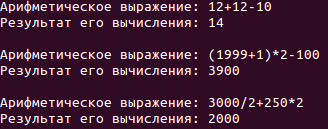
\includegraphics[scale=0.6]{images/example_calc}
\end{center}
\vspace*{-8mm}
\caption{}\label{fig:example_calc}
\end{figure}
